% الفصل 3 — الموارد البشرية: نظرة عامة ودليل الصفحات.
% كل صفحة مشروحة في صفحتها المستقلة (chapters/03-hr-features.tex)؛ لا تكرر خطواتها هنا.
\chapter{الموارد البشرية}
\label{ch:hr}

\section{ماذا ستنجز؟}

\textbf{النتيجة:} تعرف من يعمل، وفي أي وظيفة، ومتى يعمل، وكيف تراجع إجازاته وراتبه. نبدأ بسارة، ثم نطبّق الخطوات نفسها على بقية الفريق.

\textbf{من يتولى ماذا؟} الموارد البشرية: بيانات الفريق والإجازات. الموظف: حضوره. فريق الرواتب: الحسابات. المسؤول المخوّل: السياسات والأجهزة. وتعتمد المهام والمشاريع على بيانات الأشخاص والوظائف نفسها.

\begin{figure}[H]
\centering
\begin{tikzpicture}[node distance=0.7cm]
  \node[entity] (asg) {\RL{التعيينات}};
  \node[entity,below right=0.7cm and 0.5cm of asg] (mem) {\RL{الأعضاء}};
  \node[entity,below left=0.7cm and 0.5cm of asg] (pos) {\RL{المناصب}};
  \node[entityOpt,below right=0.7cm and 0.1cm of pos] (node) {\RL{الوحدات التنظيمية}};
  \node[entityOpt,below left=0.7cm and 0.1cm of pos] (loc) {\RL{النقاط الجغرافية}};
  \draw[dependsOn] (asg.south) -- ++(0,-0.3) -| (mem.north);
  \draw[dependsOn] (asg.south) -- ++(0,-0.3) -| (pos.north);
  \draw[dependsOnOpt] (pos.south) -- ++(0,-0.3) -| (node.north);
  \draw[dependsOnOpt] (pos.south) -- ++(0,-0.3) -| (loc.north);
\end{tikzpicture}
\rclegend
\caption{التعيين يربط الشخص بالوظيفة}
\label{fig:hr-models}
\end{figure}

سارة هي العضو، ومدير الموارد البشرية هو المنصب، والتعيين يربطهما. وللمنصب رابطان اختياريان: الوحدة التنظيمية (القسم) والنقطة الجغرافية (الموقع).

\section{صفحات الموارد البشرية}
\label{sec:hr-pages}

\begin{figure}[H]
\centering
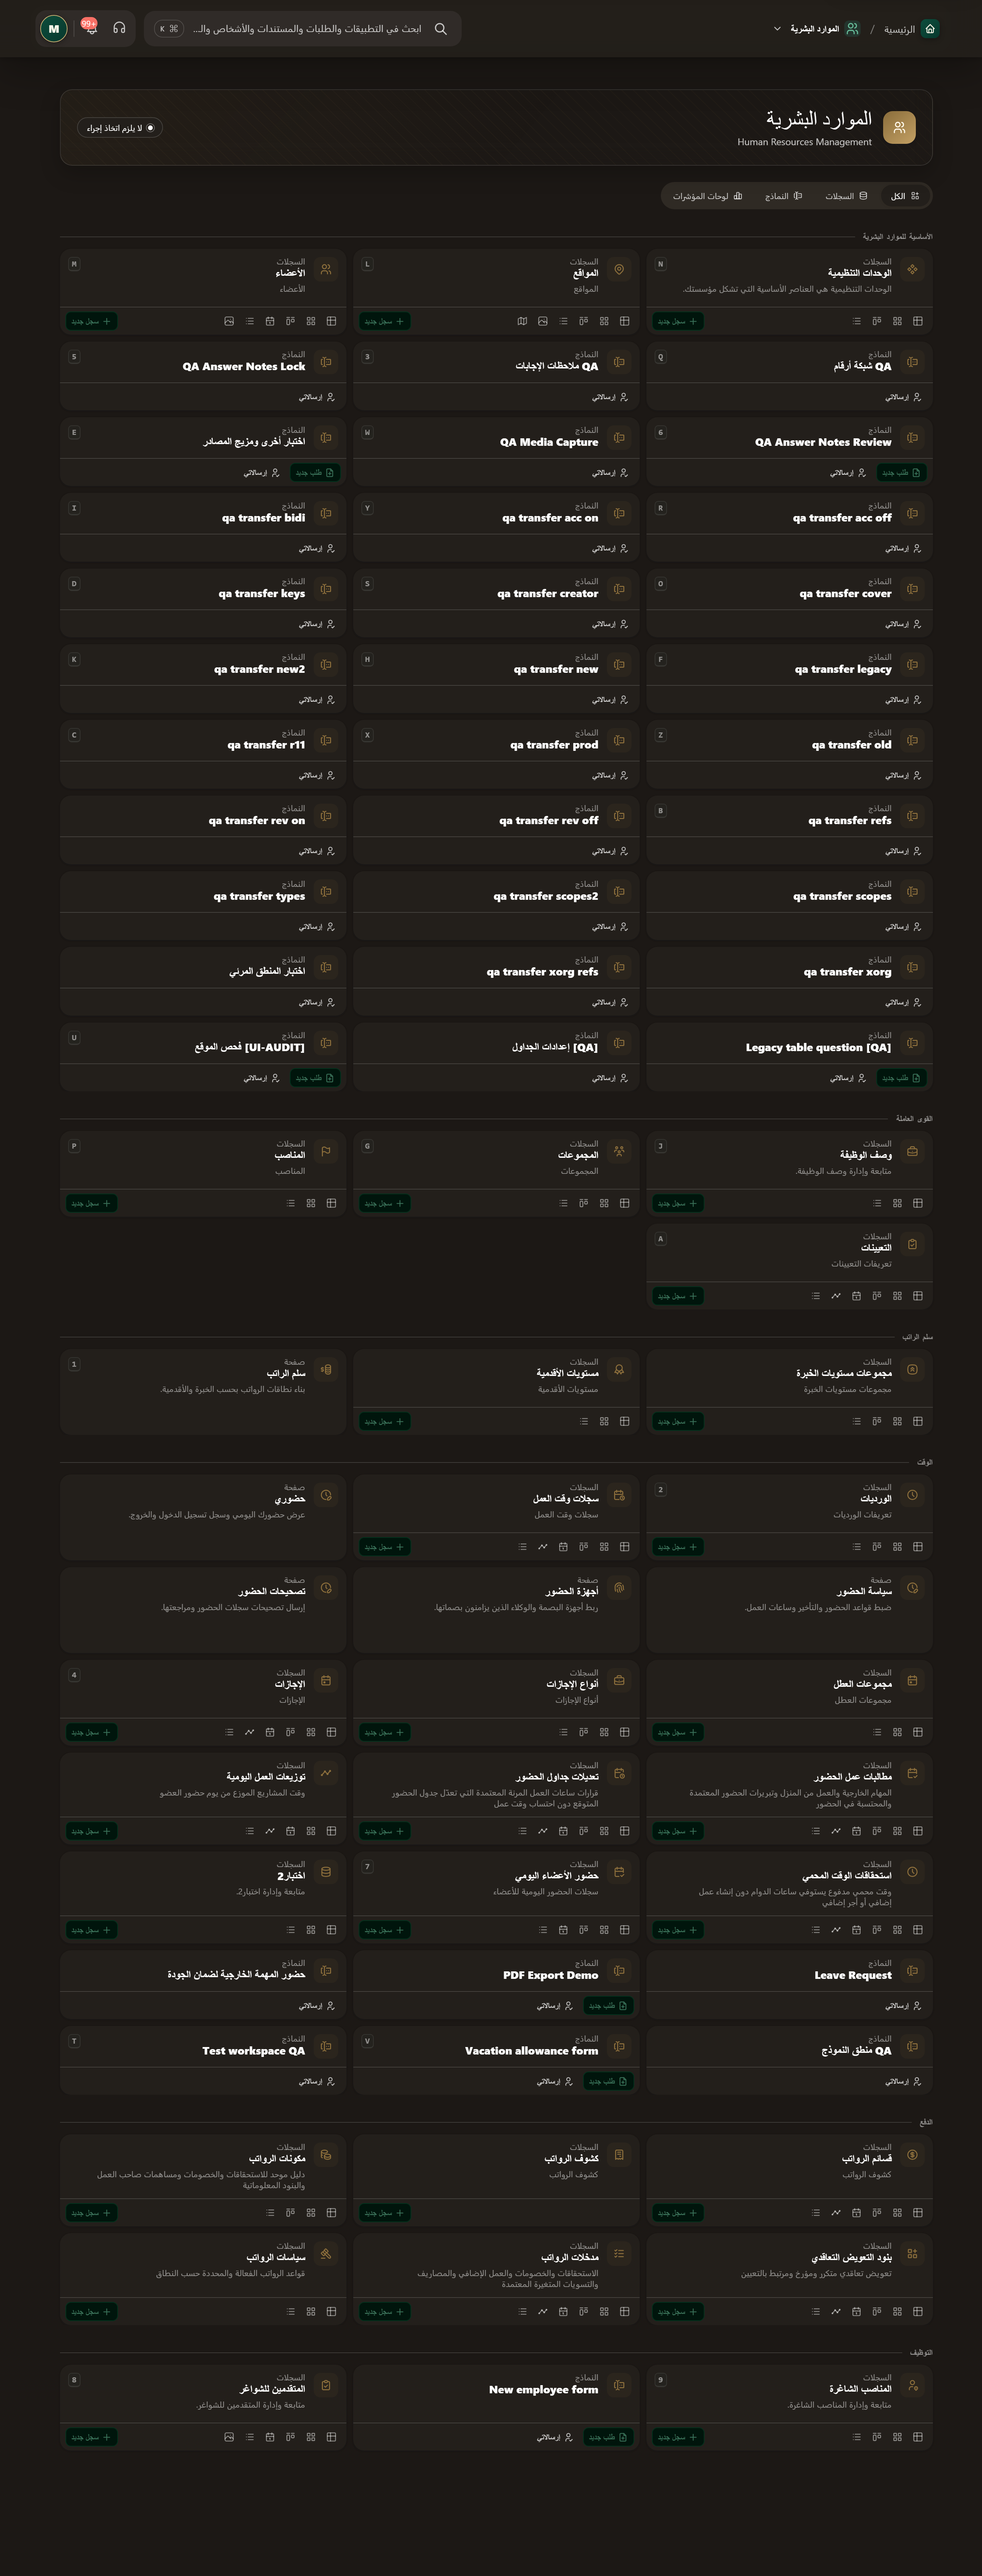
\includegraphics[width=0.95\linewidth]{figures/screens/ch03-hr-pages-clear-ar.png}
\caption{صفحات الهيكل والأشخاص}
\label{fig:hr-pages-screen}
\end{figure}

افتح الصفحات بهذا الترتيب: الأشخاص والهيكل، ثم الوقت، ثم الرواتب إن كانت مؤسستك تستخدمها. لكل صفحة شرح مستقل بالصور. \textbf{المسار:} «الموارد البشرية» / «المجموعة المذكورة مع الصفحة» / «الصفحة».

\textbf{في كل قائمة:} عرض جدول أو بطاقات أو غيرها، بحث وتصفية وعروض محفوظة، استيراد ملفات إكسل وتصديرها، وحذف جماعي؛ حسب صلاحيتك. ويذكر شرح كل صفحة ما تتميز به.

\begin{table}[H]
\centering
\caption{الأشخاص والهيكل: الأولوية الأولى}
\label{tab:hr-pages-core}
\rcZebra
\begin{tabularx}{\linewidth}{R{4.2cm} Y}
\rcHeaderRow
\thh{الصفحة ومجموعتها} & \thh{ماذا تقدم هذه الصفحة؟}\\
الأعضاء — القوى العاملة & ملف كامل لكل موظف: الهوية والاتصال والعائلة والمؤهلات والوثائق والحساب.\\
المناصب — القوى العاملة & الوظائف وتبعيتها وقسمها وموقعها ودرجتها ووردياتها.\\
التعيينات — القوى العاملة & من يشغل المنصب، ومنذ متى، وبأي عقد وراتب ووردية.\\
الوحدات التنظيمية — الأساسية & شجرة الأقسام والإدارات ومديريها.\\
النقاط الجغرافية — الأساسية & مواقع العمل وعناوينها على الخريطة.\\
المجموعات — القوى العاملة & فرق ولجان تجمع أعضاء من أقسام مختلفة.\\
\end{tabularx}
\end{table}

\begin{table}[H]
\centering
\caption{متابعة يوم العمل: صفحات الوقت}
\label{tab:hr-pages-time}
\rcZebra
\begin{tabularx}{\linewidth}{R{4.2cm} Y}
\rcHeaderRow
\thh{الصفحة ومجموعتها} & \thh{ماذا تقدم هذه الصفحة؟}\\
الورديات — الوقت & أيام العمل وساعاته واستراحاته، وكيف تصل الوردية إلى الموظف.\\
حضوري — الوقت & أيام حضورك المسجلة: الدخول والخروج والمدة.\\
جداول الدوام — الوقت & حضور الفريق لفترة تختارها.\\
أنواع الإجازات — الوقت & أنواع الإجازة وقواعدها وأثرها في الراتب.\\
الإجازات — الوقت & إجازات الموظفين: نوعها وتاريخها وحالتها.\\
مجموعات العطل الرسمية — الوقت & تقويم مشترك للعطل الرسمية، ومن يتبعه.\\
تصحيحات الحضور — الوقت & طلبات تصحيح أيام الحضور والبتّ فيها.\\
سياسة الحضور — الوقت & قواعد التأخر والخروج المبكر والعمل الإضافي.\\
أجهزة الحضور — الوقت & أجهزة البصمة وربط مستخدميها بالأعضاء.\\
\end{tabularx}
\end{table}

\begin{table}[H]
\centering
\caption{عند احتساب الرواتب: الإعداد ثم المراجعة}
\label{tab:hr-pages-pay}
\rcZebra
\begin{tabularx}{\linewidth}{R{4.2cm} Y}
\rcHeaderRow
\thh{الصفحة ومجموعتها} & \thh{ماذا تقدم هذه الصفحة؟}\\
المستويات الوظيفية — سلم الراتب & الدرجات الوظيفية وحدود رواتبها.\\
مستويات الخبرة — سلم الراتب & مجموعات الخبرة ومستوياتها وزياداتها.\\
سلم الراتب — سلم الراتب & جدول الرواتب المرجعية لكل درجة ومستوى خبرة.\\
مدخلات الرواتب — الدفع & بنود الشهر المتغيرة: مكافأة، خصم، عمل إضافي.\\
قسائم الرواتب — الدفع & حساب راتب كل موظف واعتماده.\\
كشوف الرواتب — الدفع & كشف رواتب الشهر من القسائم المعتمدة.\\
\end{tabularx}
\end{table}
